% Final report. The numbers, tables and figures come from report_numbers.tex, which
% white_advantage writes when run with --report (see README.md in the repo root).
% Build from this folder:  pdflatex -jobname=finalReport report.tex  (twice)
\documentclass[11pt,a4paper]{article}
\usepackage[a4paper,margin=2cm,top=1.8cm,bottom=2cm]{geometry}
\usepackage[T1]{fontenc}
\usepackage[sc]{mathpazo}
\linespread{1.05}
\usepackage{courier}
\usepackage[scaled=0.9]{helvet}
\usepackage{microtype}
\usepackage{xcolor}
\usepackage{graphicx}
\usepackage{booktabs}
\usepackage{tabularx}
\usepackage{enumitem}
\usepackage{amsmath}
\usepackage{caption}
\usepackage[hidelinks]{hyperref}
\usepackage{titlesec}
\usepackage{placeins}
\usepackage{pgfplots}
\pgfplotsset{compat=1.16}

\titleformat{\section}{\large\sffamily\bfseries}{\thesection.}{0.5em}{}
\titleformat{\subsection}{\normalsize\sffamily\bfseries}{\thesubsection}{0.5em}{}
\titlespacing*{\section}{0pt}{12pt}{4pt}
\titlespacing*{\subsection}{0pt}{8pt}{3pt}
\setlist{itemsep=2pt,topsep=3pt,leftmargin=1.3em}
\setlength{\parindent}{0pt}
\setlength{\parskip}{4pt}
\captionsetup{font=small,labelfont=bf}

% red placeholder for anything not filled in yet
\newcommand{\TBD}[1]{\textcolor{red}{\textbf{[#1]}}}

% placeholder: white_advantage --report report_numbers.tex replaces this file with the real numbers
\newcommand{\MonthList}{2024-01 and 2024-02}
\newcommand{\GamesRead}{190,562,735}
\newcommand{\GamesUsed}{162,175,412}
\newcommand{\PctUsed}{85.1\%}
\newcommand{\SkipNoResult}{6,007}
\newcommand{\SkipAbandoned}{502,851}
\newcommand{\SkipNoRating}{0}
\newcommand{\SkipGap}{27,878,465}
\newcommand{\FileRows}{2024-01 & 98,994,760 & 84,177,790 & 85.0\% \\
2024-02 & 91,567,975 & 77,997,622 & 85.2\% \\
}
\newcommand{\HAll}{+11.9}
\newcommand{\HAllCI}{0.1}
\newcommand{\ScoreAll}{0.517}
\newcommand{\ExpectedAll}{0.500}
\newcommand{\WhiteAll}{49.7\%}
\newcommand{\DrawAll}{4.0\%}
\newcommand{\BlackAll}{46.3\%}
\newcommand{\FigResults}{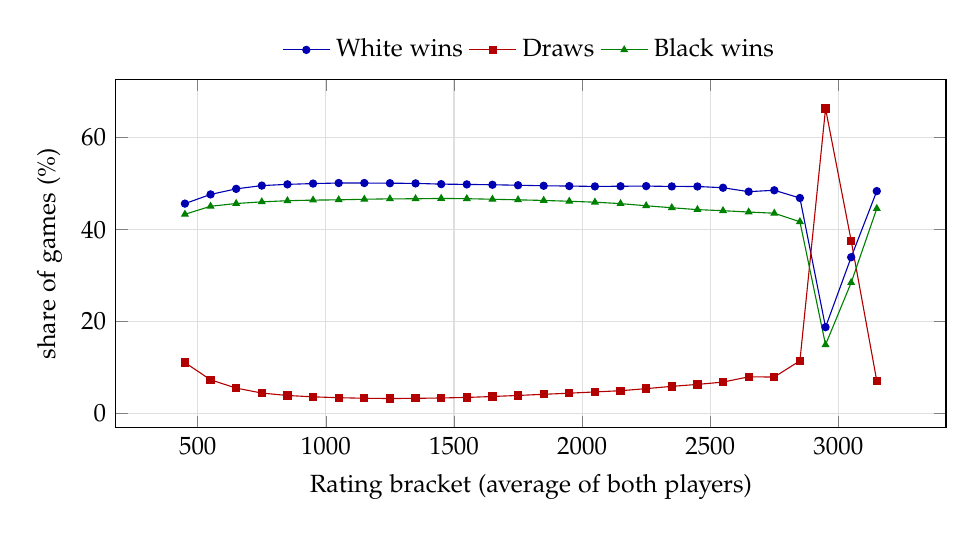
\begin{tikzpicture}
\begin{axis}[width=\linewidth, height=6cm, grid=major, grid style={gray!25},
  xlabel={Rating bracket (average of both players)}, ylabel={share of games (\%)},
  legend style={draw=none, font=\small, at={(0.5,1.02)}, anchor=south},
  legend columns=5,
  tick label style={font=\small}, label style={font=\small},
  xticklabel style={/pgf/number format/1000 sep={}}]
\addplot+[blue!70!black, mark=*, mark size=1.3pt, mark options={fill=blue!70!black}] coordinates {
(450,45.64)
(550,47.64)
(650,48.85)
(750,49.56)
(850,49.83)
(950,50.00)
(1050,50.12)
(1150,50.12)
(1250,50.08)
(1350,50.04)
(1450,49.88)
(1550,49.82)
(1650,49.74)
(1750,49.64)
(1850,49.52)
(1950,49.46)
(2050,49.38)
(2150,49.42)
(2250,49.45)
(2350,49.38)
(2450,49.37)
(2550,49.09)
(2650,48.24)
(2750,48.54)
(2850,46.86)
(2950,18.76)
(3050,33.97)
(3150,48.36)
};
\addlegendentry{White wins}
\addplot+[red!70!black, mark=square*, mark size=1.3pt, mark options={fill=red!70!black}] coordinates {
(450,11.04)
(550,7.30)
(650,5.50)
(750,4.42)
(850,3.89)
(950,3.60)
(1050,3.41)
(1150,3.29)
(1250,3.23)
(1350,3.27)
(1450,3.35)
(1550,3.47)
(1650,3.67)
(1750,3.90)
(1850,4.15)
(1950,4.39)
(2050,4.67)
(2150,4.93)
(2250,5.38)
(2350,5.88)
(2450,6.30)
(2550,6.81)
(2650,7.95)
(2750,7.91)
(2850,11.44)
(2950,66.31)
(3050,37.58)
(3150,7.07)
};
\addlegendentry{Draws}
\addplot+[green!50!black, mark=triangle*, mark size=1.3pt, mark options={fill=green!50!black}] coordinates {
(450,43.32)
(550,45.06)
(650,45.66)
(750,46.02)
(850,46.27)
(950,46.40)
(1050,46.46)
(1150,46.59)
(1250,46.68)
(1350,46.69)
(1450,46.77)
(1550,46.71)
(1650,46.59)
(1750,46.46)
(1850,46.33)
(1950,46.15)
(2050,45.95)
(2150,45.64)
(2250,45.17)
(2350,44.74)
(2450,44.33)
(2550,44.10)
(2650,43.81)
(2750,43.55)
(2850,41.70)
(2950,14.93)
(3050,28.45)
(3150,44.56)
};
\addlegendentry{Black wins}
\end{axis}
\end{tikzpicture}}
\newcommand{\OpeningRows}{King's Gambit & 2,282,379 & 1633 & 51.3\% & 3.0\% & 45.6\% & $+18.4 \pm 0.5$ \\
Evans Gambit & 165,739 & 1680 & 51.9\% & 3.3\% & 44.8\% & $+24.0 \pm 1.7$ \\
Danish Gambit & 484,805 & 1635 & 53.8\% & 3.2\% & 43.0\% & $+37.1 \pm 1.0$ \\
Smith-Morra Gambit & 1,136,895 & 1727 & 49.6\% & 3.6\% & 46.8\% & $+11.2 \pm 0.6$ \\
\midrule
Petrov's Defense & 2,071,985 & 1460 & 50.4\% & 3.9\% & 45.7\% & $+15.5 \pm 0.5$ \\
Berlin Defense & 579,944 & 1544 & 50.3\% & 5.6\% & 44.1\% & $+20.8 \pm 0.9$ \\
Queen's Gambit Declined & 3,660,887 & 1729 & 51.3\% & 4.5\% & 44.2\% & $+23.9 \pm 0.4$ \\
French Exchange & 985,286 & 1765 & 48.1\% & 4.9\% & 47.1\% & $+4.2 \pm 0.7$ \\
}
\newcommand{\OpeningDefRows}{King's Gambit & Aggressive & \emph{King's Gambit} & -- \\
Evans Gambit & Aggressive & \emph{Italian Game: Evans Gambit} & -- \\
Danish Gambit & Aggressive & \emph{Danish Gambit} & -- \\
Smith-Morra Gambit & Aggressive & \emph{Sicilian Defense: Smith-Morra Gambit} & -- \\
Petrov's Defense & Drawish & \emph{Petrov's Defense}, \emph{Russian Game} & Stafford Gambit, Cochrane Gambit \\
Berlin Defense & Drawish & \emph{Ruy Lopez: Berlin Defense} & -- \\
Queen's Gambit Declined & Drawish & \emph{Queen's Gambit Declined} & Albin Countergambit, Chigorin Defense, Baltic Defense \\
French Exchange & Drawish & \emph{French Defense: Exchange Variation} & -- \\
}
\newcommand{\OpeningGames}{11,367,920}
\newcommand{\OpeningShare}{7.0\%}
\newcommand{\GroupRows}{Aggressive (all 4) & 4,069,818 & 1662 & 51.2\% & 3.2\% & 45.6\% & $+18.8 \pm 0.3$ \\
Drawish (all 4) & 7,298,102 & 1643 & 50.5\% & 4.4\% & 45.0\% & $+18.6 \pm 0.3$ \\
Other openings & 141,698,824 & 1642 & 49.5\% & 4.0\% & 46.5\% & $+10.7 \pm 0.1$ \\
}
\newcommand{\CompareRows}{All speeds & $+18.8 \pm 0.3$ & $+18.6 \pm 0.3$ & $+0.2 \pm 0.4$ & +1.0 & $0.298$ \\
Bullet & $+16.9 \pm 0.6$ & $+16.3 \pm 0.4$ & $+0.6 \pm 0.8$ & +1.7 & $0.097$ \\
Blitz & $+19.5 \pm 0.5$ & $+18.9 \pm 0.4$ & $+0.6 \pm 0.6$ & +2.0 & $0.044$ \\
Rapid & $+20.3 \pm 0.9$ & $+22.4 \pm 0.6$ & $-2.1 \pm 1.1$ & -3.7 & $1.8 \times 10^{-4}$ \\
}
\newcommand{\CompareDiff}{$+0.2 \pm 0.4$}
\newcommand{\CompareZ}{1.0}
\newcommand{\CompareP}{$0.298$}
\newcommand{\FigOpenings}{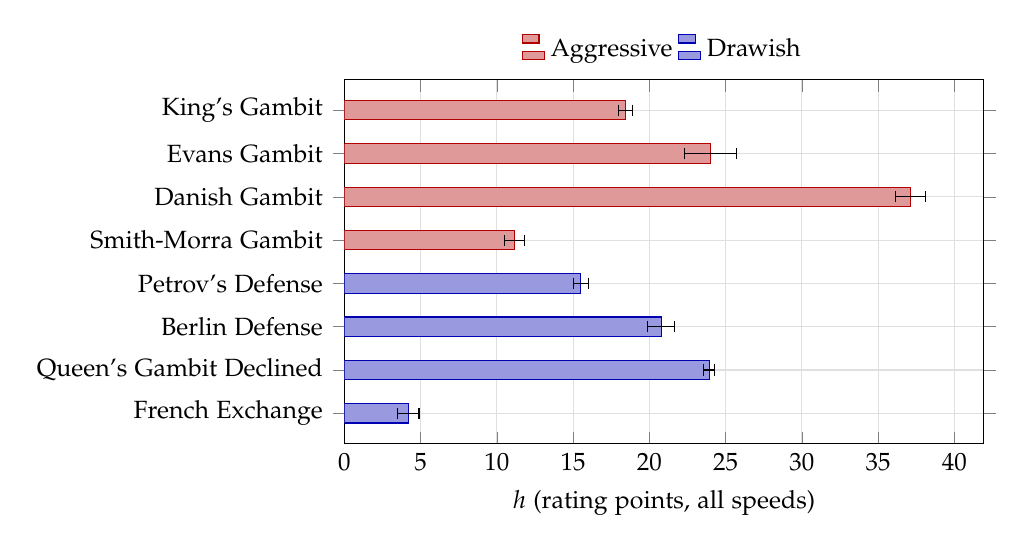
\begin{tikzpicture}
\begin{axis}[xbar, bar width=7pt, width=0.8\linewidth, height=6.2cm, xmin=0.0,
  ytick={1,...,8}, yticklabels={{French Exchange},{Queen's Gambit Declined},{Berlin Defense},{Petrov's Defense},{Smith-Morra Gambit},{Danish Gambit},{Evans Gambit},{King's Gambit}},
  xlabel={$h$ (rating points, all speeds)}, grid=major, grid style={gray!25},
  tick label style={font=\small}, label style={font=\small},
  legend style={draw=none, font=\small, at={(0.5,1.02)}, anchor=south},
  legend columns=2]
\addplot+[bar shift=0pt, draw=red!70!black, fill=red!70!black!40, error bars/.cd, x dir=both, x explicit, error bar style={black}] coordinates {
(18.43,8) +- (0.45,0)
(24.01,7) +- (1.69,0)
(37.12,6) +- (0.99,0)
(11.15,5) +- (0.64,0)
};
\addlegendentry{Aggressive}
\addplot+[bar shift=0pt, draw=blue!70!black, fill=blue!70!black!40, error bars/.cd, x dir=both, x explicit, error bar style={black}] coordinates {
(15.51,4) +- (0.48,0)
(20.77,3) +- (0.90,0)
(23.92,2) +- (0.36,0)
(4.20,1) +- (0.69,0)
};
\addlegendentry{Drawish}
\end{axis}
\end{tikzpicture}}
\newcommand{\FigGroupH}{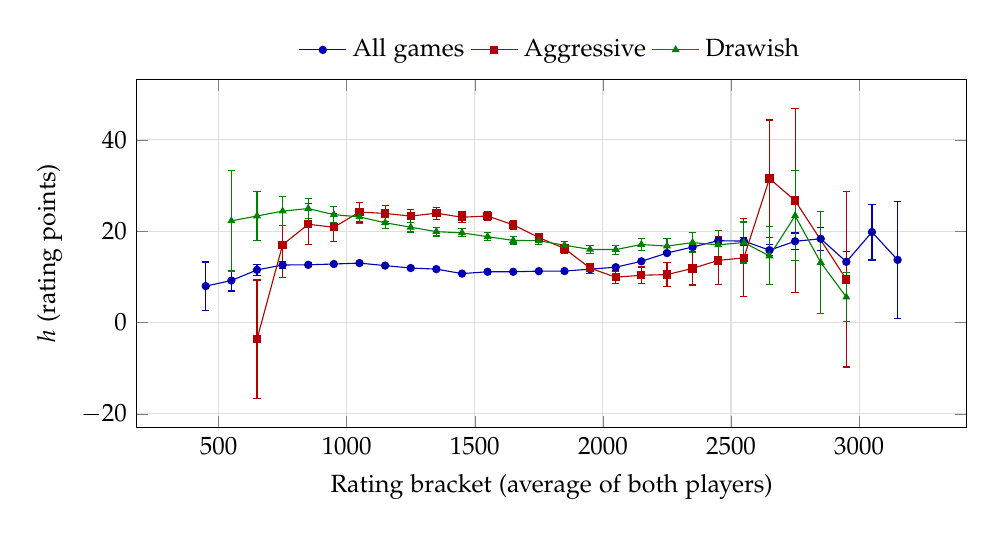
\begin{tikzpicture}
\begin{axis}[width=\linewidth, height=6cm, grid=major, grid style={gray!25},
  xlabel={Rating bracket (average of both players)}, ylabel={$h$ (rating points)},
  legend style={draw=none, font=\small, at={(0.5,1.02)}, anchor=south},
  legend columns=5,
  tick label style={font=\small}, label style={font=\small},
  xticklabel style={/pgf/number format/1000 sep={}}]
\addplot+[blue!70!black, mark=*, mark size=1.3pt, mark options={fill=blue!70!black}, error bars/.cd, y dir=both, y explicit, error bar style={blue!70!black}] coordinates {
(450,7.99) +- (0,5.29)
(550,9.21) +- (0,2.29)
(650,11.54) +- (0,1.16)
(750,12.61) +- (0,0.69)
(850,12.66) +- (0,0.47)
(950,12.83) +- (0,0.35)
(1050,13.03) +- (0,0.28)
(1150,12.48) +- (0,0.25)
(1250,11.95) +- (0,0.22)
(1350,11.71) +- (0,0.20)
(1450,10.73) +- (0,0.18)
(1550,11.13) +- (0,0.17)
(1650,11.13) +- (0,0.17)
(1750,11.27) +- (0,0.17)
(1850,11.29) +- (0,0.17)
(1950,11.70) +- (0,0.19)
(2050,12.13) +- (0,0.21)
(2150,13.42) +- (0,0.26)
(2250,15.23) +- (0,0.33)
(2350,16.55) +- (0,0.44)
(2450,17.93) +- (0,0.60)
(2550,17.85) +- (0,0.85)
(2650,15.86) +- (0,1.22)
(2750,17.81) +- (0,1.81)
(2850,18.35) +- (0,2.47)
(2950,13.31) +- (0,2.30)
(3050,19.83) +- (0,6.12)
(3150,13.73) +- (0,12.87)
};
\addlegendentry{All games}
\addplot+[red!70!black, mark=square*, mark size=1.3pt, mark options={fill=red!70!black}, error bars/.cd, y dir=both, y explicit, error bar style={red!70!black}] coordinates {
(650,-3.65) +- (0,12.98)
(750,17.04) +- (0,7.19)
(850,21.53) +- (0,4.48)
(950,20.88) +- (0,3.04)
(1050,24.21) +- (0,2.18)
(1150,23.91) +- (0,1.77)
(1250,23.32) +- (0,1.48)
(1350,23.96) +- (0,1.29)
(1450,23.07) +- (0,1.14)
(1550,23.35) +- (0,1.04)
(1650,21.40) +- (0,0.98)
(1750,18.63) +- (0,0.95)
(1850,16.22) +- (0,0.98)
(1950,11.92) +- (0,1.10)
(2050,9.94) +- (0,1.36)
(2150,10.37) +- (0,1.80)
(2250,10.51) +- (0,2.57)
(2350,11.87) +- (0,3.64)
(2450,13.62) +- (0,5.27)
(2550,14.18) +- (0,8.54)
(2650,31.54) +- (0,12.82)
(2750,26.71) +- (0,20.15)
(2950,9.47) +- (0,19.19)
};
\addlegendentry{Aggressive}
\addplot+[green!50!black, mark=triangle*, mark size=1.3pt, mark options={fill=green!50!black}, error bars/.cd, y dir=both, y explicit, error bar style={green!50!black}] coordinates {
(550,22.29) +- (0,10.99)
(650,23.34) +- (0,5.36)
(750,24.41) +- (0,3.21)
(850,24.98) +- (0,2.23)
(950,23.64) +- (0,1.69)
(1050,23.15) +- (0,1.36)
(1150,21.86) +- (0,1.19)
(1250,20.89) +- (0,1.05)
(1350,19.92) +- (0,0.95)
(1450,19.65) +- (0,0.88)
(1550,18.82) +- (0,0.82)
(1650,18.00) +- (0,0.79)
(1750,17.93) +- (0,0.77)
(1850,16.94) +- (0,0.79)
(1950,16.03) +- (0,0.85)
(2050,15.99) +- (0,0.99)
(2150,17.10) +- (0,1.23)
(2250,16.75) +- (0,1.66)
(2350,17.52) +- (0,2.25)
(2450,17.02) +- (0,3.08)
(2550,17.54) +- (0,4.50)
(2650,14.60) +- (0,6.35)
(2750,23.39) +- (0,9.85)
(2850,13.18) +- (0,11.13)
(2950,5.58) +- (0,5.42)
};
\addlegendentry{Drawish}
\end{axis}
\end{tikzpicture}}
\newcommand{\FigGroupDraws}{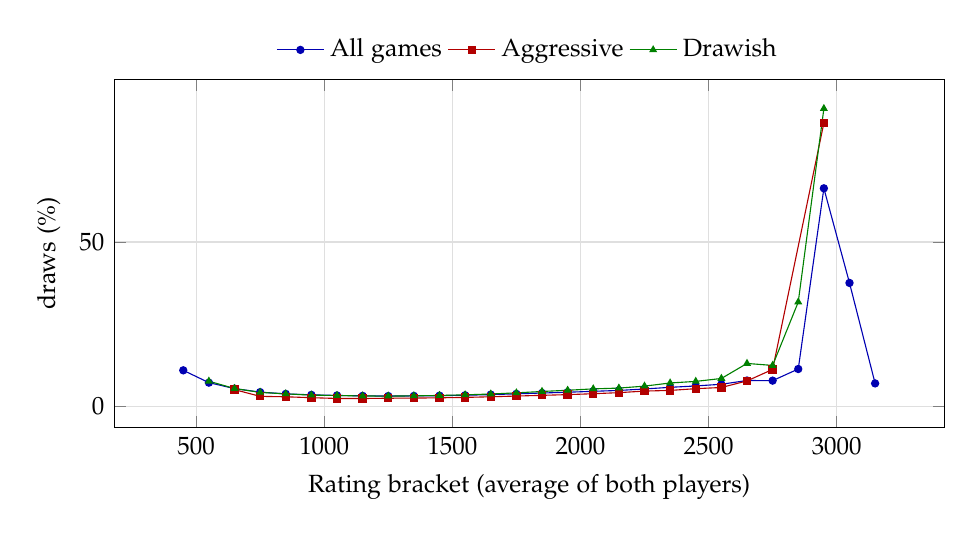
\begin{tikzpicture}
\begin{axis}[width=\linewidth, height=6cm, grid=major, grid style={gray!25},
  xlabel={Rating bracket (average of both players)}, ylabel={draws (\%)},
  legend style={draw=none, font=\small, at={(0.5,1.02)}, anchor=south},
  legend columns=5,
  tick label style={font=\small}, label style={font=\small},
  xticklabel style={/pgf/number format/1000 sep={}}]
\addplot+[blue!70!black, mark=*, mark size=1.3pt, mark options={fill=blue!70!black}] coordinates {
(450,11.04)
(550,7.30)
(650,5.50)
(750,4.42)
(850,3.89)
(950,3.60)
(1050,3.41)
(1150,3.29)
(1250,3.23)
(1350,3.27)
(1450,3.35)
(1550,3.47)
(1650,3.67)
(1750,3.90)
(1850,4.15)
(1950,4.39)
(2050,4.67)
(2150,4.93)
(2250,5.38)
(2350,5.88)
(2450,6.30)
(2550,6.81)
(2650,7.95)
(2750,7.91)
(2850,11.44)
(2950,66.31)
(3050,37.58)
(3150,7.07)
};
\addlegendentry{All games}
\addplot+[red!70!black, mark=square*, mark size=1.3pt, mark options={fill=red!70!black}] coordinates {
(650,5.18)
(750,3.14)
(850,3.01)
(950,2.73)
(1050,2.50)
(1150,2.48)
(1250,2.57)
(1350,2.61)
(1450,2.70)
(1550,2.82)
(1650,3.01)
(1750,3.23)
(1850,3.45)
(1950,3.66)
(2050,3.94)
(2150,4.26)
(2250,4.74)
(2350,4.94)
(2450,5.47)
(2550,5.83)
(2650,7.82)
(2750,11.32)
(2950,86.15)
};
\addlegendentry{Aggressive}
\addplot+[green!50!black, mark=triangle*, mark size=1.3pt, mark options={fill=green!50!black}] coordinates {
(550,7.74)
(650,5.51)
(750,4.35)
(850,3.89)
(950,3.51)
(1050,3.40)
(1150,3.25)
(1250,3.21)
(1350,3.29)
(1450,3.41)
(1550,3.60)
(1650,3.85)
(1750,4.20)
(1850,4.62)
(1950,4.99)
(2050,5.41)
(2150,5.65)
(2250,6.24)
(2350,7.20)
(2450,7.68)
(2550,8.57)
(2650,13.13)
(2750,12.53)
(2850,31.77)
(2950,90.51)
};
\addlegendentry{Drawish}
\end{axis}
\end{tikzpicture}}
\newcommand{\SpeedRows}{All speeds & 162,175,412 & 1638 & 49.7\% & 4.0\% & 46.3\% & $+11.9 \pm 0.1$ \\
UltraBullet & 722,976 & 1611 & 50.3\% & 2.0\% & 47.8\% & $+9.1 \pm 0.8$ \\
Bullet & 59,945,392 & 1716 & 49.9\% & 3.0\% & 47.1\% & $+9.9 \pm 0.1$ \\
Blitz & 77,918,475 & 1613 & 49.6\% & 4.4\% & 46.0\% & $+12.8 \pm 0.1$ \\
Rapid & 22,650,621 & 1520 & 49.6\% & 4.9\% & 45.5\% & $+14.2 \pm 0.1$ \\
Classical & 857,174 & 1569 & 49.1\% & 5.7\% & 45.2\% & $+13.4 \pm 0.7$ \\
Correspondence & 80,774 & 1789 & 47.5\% & 5.7\% & 46.8\% & $+2.8 \pm 2.4$ \\
}
\newcommand{\SpeedStepRows}{Bullet vs UltraBullet & $+9.9 \pm 0.1$ & $+9.1 \pm 0.8$ & $+0.8 \pm 0.8$ & +1.9 & $0.060$ \\
Blitz vs Bullet & $+12.8 \pm 0.1$ & $+9.9 \pm 0.1$ & $+2.9 \pm 0.1$ & +47.8 & $< 10^{-300}$ \\
Rapid vs Blitz & $+14.2 \pm 0.1$ & $+12.8 \pm 0.1$ & $+1.4 \pm 0.2$ & +16.9 & $9.6 \times 10^{-64}$ \\
Classical vs Rapid & $+13.4 \pm 0.7$ & $+14.2 \pm 0.1$ & $-0.8 \pm 0.8$ & -2.0 & $0.042$ \\
Correspondence vs Classical & $+2.8 \pm 2.4$ & $+13.4 \pm 0.7$ & $-10.6 \pm 2.5$ & -8.2 & $2.3 \times 10^{-16}$ \\
}
\newcommand{\FigSpeed}{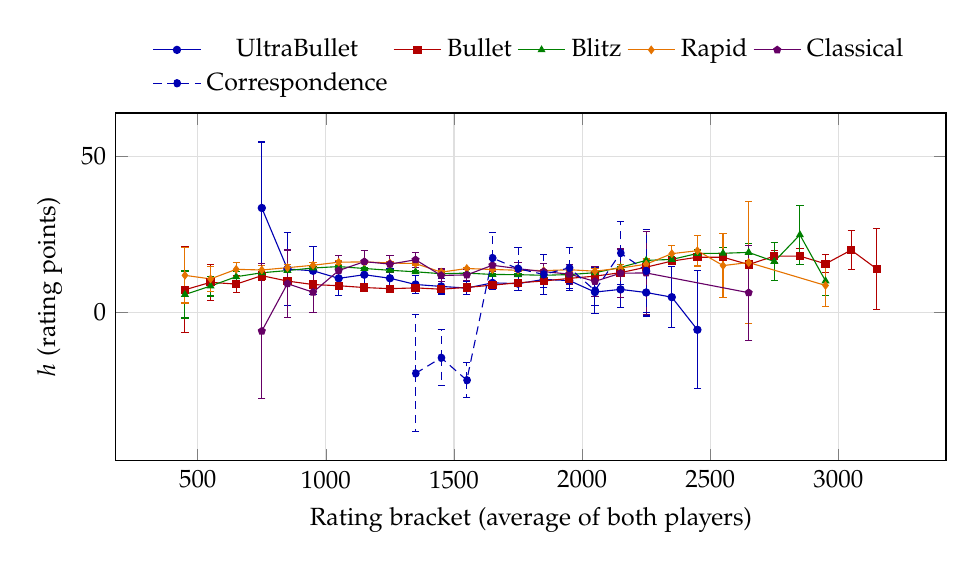
\begin{tikzpicture}
\begin{axis}[width=\linewidth, height=6cm, grid=major, grid style={gray!25},
  xlabel={Rating bracket (average of both players)}, ylabel={$h$ (rating points)},
  legend style={draw=none, font=\small, at={(0.5,1.02)}, anchor=south},
  legend columns=5,
  tick label style={font=\small}, label style={font=\small},
  xticklabel style={/pgf/number format/1000 sep={}}]
\addplot+[blue!70!black, mark=*, mark size=1.3pt, mark options={fill=blue!70!black}, error bars/.cd, y dir=both, y explicit, error bar style={blue!70!black}] coordinates {
(750,33.37) +- (0,21.15)
(850,13.80) +- (0,11.76)
(950,13.24) +- (0,7.75)
(1050,10.81) +- (0,5.41)
(1150,11.97) +- (0,4.28)
(1250,10.84) +- (0,3.22)
(1350,8.84) +- (0,2.81)
(1450,8.22) +- (0,2.44)
(1550,7.70) +- (0,2.20)
(1650,9.36) +- (0,2.07)
(1750,9.11) +- (0,2.27)
(1850,10.45) +- (0,2.54)
(1950,10.11) +- (0,3.08)
(2050,6.41) +- (0,4.18)
(2150,7.27) +- (0,5.87)
(2250,6.27) +- (0,7.54)
(2350,4.78) +- (0,9.71)
(2450,-5.68) +- (0,18.95)
};
\addlegendentry{UltraBullet}
\addplot+[red!70!black, mark=square*, mark size=1.3pt, mark options={fill=red!70!black}, error bars/.cd, y dir=both, y explicit, error bar style={red!70!black}] coordinates {
(450,7.15) +- (0,13.78)
(550,9.53) +- (0,5.86)
(650,8.97) +- (0,2.67)
(750,11.67) +- (0,1.45)
(850,9.94) +- (0,0.94)
(950,8.82) +- (0,0.67)
(1050,8.45) +- (0,0.52)
(1150,7.86) +- (0,0.44)
(1250,7.50) +- (0,0.39)
(1350,7.75) +- (0,0.35)
(1450,7.33) +- (0,0.32)
(1550,7.91) +- (0,0.30)
(1650,8.62) +- (0,0.29)
(1750,9.39) +- (0,0.28)
(1850,9.95) +- (0,0.28)
(1950,10.80) +- (0,0.29)
(2050,11.51) +- (0,0.32)
(2150,12.63) +- (0,0.36)
(2250,14.39) +- (0,0.44)
(2350,16.34) +- (0,0.55)
(2450,17.58) +- (0,0.71)
(2550,17.58) +- (0,0.97)
(2650,15.24) +- (0,1.35)
(2750,17.93) +- (0,1.90)
(2850,17.93) +- (0,2.56)
(2950,15.46) +- (0,2.88)
(3050,19.87) +- (0,6.15)
(3150,13.82) +- (0,12.87)
};
\addlegendentry{Bullet}
\addplot+[green!50!black, mark=triangle*, mark size=1.3pt, mark options={fill=green!50!black}, error bars/.cd, y dir=both, y explicit, error bar style={green!50!black}] coordinates {
(450,5.63) +- (0,7.52)
(550,8.34) +- (0,3.18)
(650,11.33) +- (0,1.61)
(750,12.60) +- (0,0.96)
(850,13.31) +- (0,0.65)
(950,14.13) +- (0,0.49)
(1050,14.58) +- (0,0.40)
(1150,13.97) +- (0,0.35)
(1250,13.39) +- (0,0.31)
(1350,12.91) +- (0,0.28)
(1450,12.30) +- (0,0.26)
(1550,12.48) +- (0,0.25)
(1650,12.06) +- (0,0.24)
(1750,11.99) +- (0,0.24)
(1850,11.79) +- (0,0.24)
(1950,12.02) +- (0,0.27)
(2050,12.62) +- (0,0.31)
(2150,14.34) +- (0,0.40)
(2250,16.57) +- (0,0.55)
(2350,16.87) +- (0,0.77)
(2450,18.78) +- (0,1.13)
(2550,18.85) +- (0,1.75)
(2650,19.12) +- (0,2.90)
(2750,16.21) +- (0,6.16)
(2850,24.75) +- (0,9.41)
(2950,9.98) +- (0,4.60)
};
\addlegendentry{Blitz}
\addplot+[orange!90!black, mark=diamond*, mark size=1.3pt, mark options={fill=orange!90!black}, error bars/.cd, y dir=both, y explicit, error bar style={orange!90!black}] coordinates {
(450,11.77) +- (0,8.86)
(550,10.63) +- (0,4.01)
(650,13.70) +- (0,2.16)
(750,13.49) +- (0,1.40)
(850,14.23) +- (0,0.99)
(950,15.00) +- (0,0.78)
(1050,15.98) +- (0,0.64)
(1150,16.09) +- (0,0.57)
(1250,15.73) +- (0,0.51)
(1350,15.56) +- (0,0.48)
(1450,12.79) +- (0,0.45)
(1550,13.96) +- (0,0.44)
(1650,13.65) +- (0,0.44)
(1750,13.41) +- (0,0.45)
(1850,13.28) +- (0,0.49)
(1950,13.57) +- (0,0.56)
(2050,13.10) +- (0,0.74)
(2150,14.10) +- (0,1.06)
(2250,15.35) +- (0,1.66)
(2350,18.72) +- (0,2.76)
(2450,19.67) +- (0,4.89)
(2550,14.90) +- (0,10.25)
(2650,15.88) +- (0,19.47)
(2950,8.53) +- (0,6.82)
};
\addlegendentry{Rapid}
\addplot+[violet!80!black, mark=pentagon*, mark size=1.3pt, mark options={fill=violet!80!black}, error bars/.cd, y dir=both, y explicit, error bar style={violet!80!black}] coordinates {
(750,-6.08) +- (0,21.70)
(850,9.10) +- (0,10.79)
(950,6.37) +- (0,6.53)
(1050,13.31) +- (0,4.78)
(1150,16.16) +- (0,3.71)
(1250,15.37) +- (0,2.81)
(1350,16.76) +- (0,2.42)
(1450,11.73) +- (0,2.07)
(1550,11.91) +- (0,1.82)
(1650,15.01) +- (0,1.94)
(1750,13.92) +- (0,2.10)
(1850,12.96) +- (0,2.47)
(1950,12.17) +- (0,3.16)
(2050,9.84) +- (0,4.86)
(2150,12.46) +- (0,7.76)
(2250,12.54) +- (0,13.27)
(2650,6.21) +- (0,15.21)
};
\addlegendentry{Classical}
\addplot+[blue!70!black, mark=*, mark size=1.3pt, mark options={fill=blue!70!black}, error bars/.cd, y dir=both, y explicit, error bar style={blue!70!black}] coordinates {
(1350,-19.66) +- (0,18.75)
(1450,-14.66) +- (0,8.94)
(1550,-21.84) +- (0,5.68)
(1650,17.32) +- (0,8.30)
(1750,13.90) +- (0,6.90)
(1850,12.07) +- (0,6.38)
(1950,14.18) +- (0,6.55)
(2050,6.91) +- (0,7.43)
(2150,18.90) +- (0,10.03)
(2250,13.20) +- (0,13.30)
};
\addlegendentry{Correspondence}
\end{axis}
\end{tikzpicture}}
\newcommand{\FigSpeedBars}{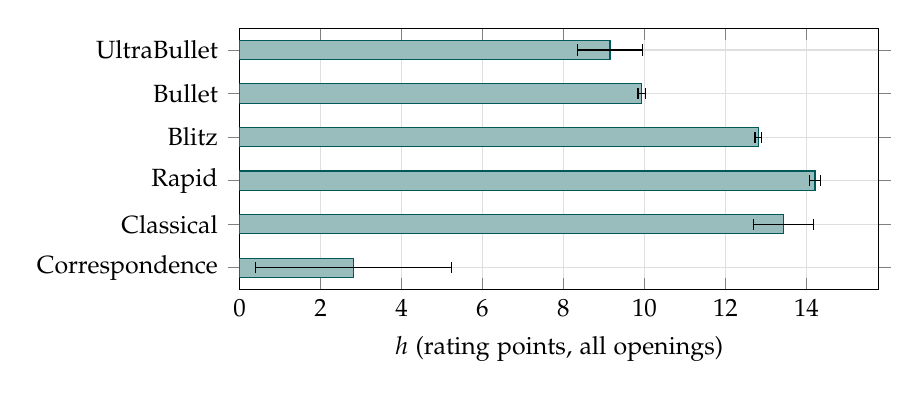
\begin{tikzpicture}
\begin{axis}[xbar, bar width=7pt, width=0.8\linewidth, height=4.9cm, xmin=0.0,
  ytick={1,...,6}, yticklabels={{Correspondence},{Classical},{Rapid},{Blitz},{Bullet},{UltraBullet}},
  xlabel={$h$ (rating points, all openings)}, grid=major, grid style={gray!25},
  tick label style={font=\small}, label style={font=\small},
  legend style={draw=none, font=\small, at={(0.5,1.02)}, anchor=south},
  legend columns=2]
\addplot+[bar shift=0pt, draw=teal!70!black, fill=teal!70!black!40, error bars/.cd, x dir=both, x explicit, error bar style={black}] coordinates {
(9.15,6) +- (0.81,0)
(9.93,5) +- (0.09,0)
(12.81,4) +- (0.08,0)
(14.21,3) +- (0.14,0)
(13.43,2) +- (0.74,0)
(2.82,1) +- (2.42,0)
};
\end{axis}
\end{tikzpicture}}
\newcommand{\FigSpeedDraws}{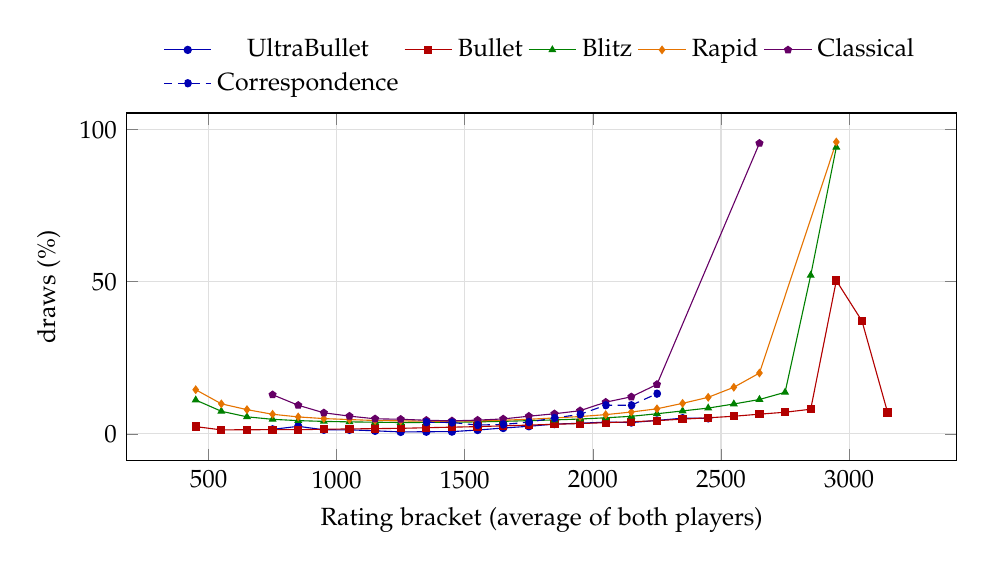
\begin{tikzpicture}
\begin{axis}[width=\linewidth, height=6cm, grid=major, grid style={gray!25},
  xlabel={Rating bracket (average of both players)}, ylabel={draws (\%)},
  legend style={draw=none, font=\small, at={(0.5,1.02)}, anchor=south},
  legend columns=5,
  tick label style={font=\small}, label style={font=\small},
  xticklabel style={/pgf/number format/1000 sep={}}]
\addplot+[blue!70!black, mark=*, mark size=1.3pt, mark options={fill=blue!70!black}] coordinates {
(750,1.49)
(850,2.49)
(950,1.35)
(1050,1.34)
(1150,1.01)
(1250,0.65)
(1350,0.71)
(1450,0.75)
(1550,1.27)
(1650,1.93)
(1750,2.50)
(1850,3.22)
(1950,3.50)
(2050,3.87)
(2150,3.73)
(2250,4.42)
(2350,5.17)
(2450,5.11)
};
\addlegendentry{UltraBullet}
\addplot+[red!70!black, mark=square*, mark size=1.3pt, mark options={fill=red!70!black}] coordinates {
(450,2.39)
(550,1.32)
(650,1.37)
(750,1.39)
(850,1.39)
(950,1.52)
(1050,1.63)
(1150,1.73)
(1250,1.83)
(1350,2.03)
(1450,2.21)
(1550,2.39)
(1650,2.65)
(1750,2.89)
(1850,3.17)
(1950,3.40)
(2050,3.70)
(2150,3.98)
(2250,4.35)
(2350,4.85)
(2450,5.29)
(2550,5.80)
(2650,6.48)
(2750,7.12)
(2850,8.10)
(2950,50.37)
(3050,37.11)
(3150,7.08)
};
\addlegendentry{Bullet}
\addplot+[green!50!black, mark=triangle*, mark size=1.3pt, mark options={fill=green!50!black}] coordinates {
(450,11.13)
(550,7.44)
(650,5.61)
(750,4.79)
(850,4.36)
(950,4.11)
(1050,3.95)
(1150,3.84)
(1250,3.74)
(1350,3.77)
(1450,3.84)
(1550,3.95)
(1650,4.13)
(1750,4.35)
(1850,4.60)
(1950,4.89)
(2050,5.29)
(2150,5.78)
(2250,6.62)
(2350,7.55)
(2450,8.48)
(2550,9.83)
(2650,11.30)
(2750,13.67)
(2850,52.10)
(2950,94.20)
};
\addlegendentry{Blitz}
\addplot+[orange!90!black, mark=diamond*, mark size=1.3pt, mark options={fill=orange!90!black}] coordinates {
(450,14.52)
(550,9.88)
(650,7.97)
(750,6.45)
(850,5.58)
(950,5.03)
(1050,4.71)
(1150,4.40)
(1250,4.29)
(1350,4.17)
(1450,4.16)
(1550,4.25)
(1650,4.49)
(1750,4.81)
(1850,5.24)
(1950,5.70)
(2050,6.33)
(2150,7.19)
(2250,8.25)
(2350,10.04)
(2450,12.02)
(2550,15.32)
(2650,20.00)
(2950,95.92)
};
\addlegendentry{Rapid}
\addplot+[violet!80!black, mark=pentagon*, mark size=1.3pt, mark options={fill=violet!80!black}] coordinates {
(750,12.87)
(850,9.41)
(950,6.93)
(1050,5.84)
(1150,4.96)
(1250,4.81)
(1350,4.48)
(1450,4.29)
(1550,4.52)
(1650,4.92)
(1750,5.81)
(1850,6.61)
(1950,7.62)
(2050,10.42)
(2150,12.19)
(2250,16.25)
(2650,95.50)
};
\addlegendentry{Classical}
\addplot+[blue!70!black, mark=*, mark size=1.3pt, mark options={fill=blue!70!black}] coordinates {
(1350,3.83)
(1450,3.74)
(1550,2.91)
(1650,3.11)
(1750,3.88)
(1850,5.23)
(1950,6.41)
(2050,9.43)
(2150,9.41)
(2250,13.22)
};
\addlegendentry{Correspondence}
\end{axis}
\end{tikzpicture}}


\begin{document}

\begin{center}
{\LARGE\bfseries The Perks of Being a First Mover}\\[4pt]
{\large Does White's Advantage in Chess Change with Rating, Opening and Time Control?}\\[6pt]
CS215 Open Project \quad$\cdot$\quad Final Report \quad$\cdot$\quad Group 02\\[2pt]
{\small Sanidhya (25b0944), Daksh Maahor (25b0974), Sahil (25b0991), VadaPavJai (25b1030)}\\[2pt]
{\small Mentor: Namish Bansal}\\[2pt]
{\small\url{https://github.com/cs215-cse-iitb/dai-aug-2026-openproject-group-2}}
\end{center}

%=====================================================================
% SECTION 1: META INFORMATION
%=====================================================================

\section*{Section 1: Meta Information}

\renewcommand{\arraystretch}{1.35}
\begin{tabularx}{\linewidth}{@{}p{4.6cm}X@{}}
\toprule
\textbf{1. Open Project Title} & The Perks of Being a First Mover: Does White's Advantage in Chess Change with Rating, Opening and Time Control? \\
\textbf{2. Group ID} & ``02'' \\
\textbf{3. Mentor Name} & Namish Bansal \\
\textbf{4. Group Members and Roll Numbers} &
  Sanidhya (25b0944); Daksh Maahor (25b0974); Sahil (25b0991); VadaPavJai (25b1030) \\
\textbf{5. Honor Code and Discussions} &
  None \\
\textbf{6. LLM Usage Links} &
\begin{minipage}[t]{\linewidth}\footnotesize
\begin{itemize}[leftmargin=1em,itemsep=0pt,topsep=0pt]
\item \url{https://claude.ai/share/041dbe60-e304-4ada-bc7e-8d070f0b5a94}
\item \url{https://claude.ai/share/1bb9222d-6e23-4b2d-8803-6cdff0f0e31c}
\end{itemize}
\end{minipage} \\
\textbf{7. Video Presentation} & \TBD{link to video} \\
\textbf{8. GitHub Repository} & \url{https://github.com/cs215-cse-iitb/dai-aug-2026-openproject-group-2} \\
\textbf{9. GitHub Handles and Initial Commit} & \\
\hspace{1em}Sanidhya & \url{https://github.com/SS3642} \quad earliest commit: October 21, 2026 \\
\hspace{1em}Daksh Maahor & \url{https://github.com/Daksh-Maahor} \quad earliest commit: November 3, 2026 \\
\hspace{1em}Sahil & \url{https://github.com/Sahil-Deo-IITB} \quad earliest commit: November 3, 2026 \\
\hspace{1em}VadaPavJai & \url{https://github.com/nauseated-potato} \quad earliest commit: October 18, 2026 \\
\textbf{10. Contribution Breakdown} &
  Unequal (25b0944: 100\%, 25b0974: 100\%, 25b0991: 100\%, 25b1030: 100\%, LLM: 25\%)\\
\bottomrule
\end{tabularx}

\vspace{8pt}
\textbf{Work split (for reference)}

\begin{tabularx}{\linewidth}{@{}>{\raggedright\arraybackslash}p{2.8cm}X@{}}
Sanidhya & Statistical modelling: fitting $h$, confidence intervals and the $z$-tests. \\
Daksh Maahor & Data cleaning and opening classification; win/draw/loss rates. \\
Sahil & Data engineering: the C++ streaming parser and the Colab pipeline. \\
VadaPavJai & Visualisation: figures, the Plotly dashboard and the report. \\
Claude & Literature review and initial analysis. \\
\end{tabularx}

\newpage

%=====================================================================
% SECTION 2: TECHNICAL CONTENT
%=====================================================================

\section*{Section 2: Technical Content}

\subsection*{Core Problem Statement}
We measure the first-move advantage on Lichess. Instead of raw win rates, we fit White's
advantage as a number of \emph{rating points}, $h$, after correcting each game for the rating
gap between the players. Under the Elo model a player $d$ points above the opponent scores
$E(d)=1/(1+10^{-d/400})$; we give White an extra $h$ points,
$E_i(h)=1/(1+10^{-(R^{\mathrm W}_i+h-R^{\mathrm B}_i)/400})$, and choose the $h$ that makes
expected scores equal actual scores ($S_i=1,\tfrac12,0$). This is the maximum-likelihood
estimate (Newton's method; standard error from the Fisher information). Overall,
$h = \HAll \pm \HAllCI$ rating points. We test three hypotheses:
\begin{itemize}
\item \textbf{H1 (Rating).} $h$ peaks at intermediate ratings and shrinks at 2200+.
\item \textbf{H2 (Openings).} Four aggressive 1.e4 gambits (King's, Evans, Danish, Smith-Morra)
  carry a larger $h$ than four drawish openings (Petrov, Berlin, QGD, French Exchange), and the
  drawish ones have more draws at every rating.
\item \textbf{H3 (Time control).} $h$ grows from Bullet to Classical.
\end{itemize}

\subsection*{Data Source(s)}
Lichess Open Database (\url{https://database.lichess.org}, CC0), standard rated games for
\MonthList: one zstd-compressed PGN per month, tens of GB each, openly downloadable. We use
seven of ~17 header tags: \texttt{Result}, \texttt{WhiteElo}, \texttt{BlackElo},
\texttt{Event}, \texttt{TimeControl}, \texttt{Termination}, \texttt{Opening}. We read
\GamesRead{} games and keep \GamesUsed{} (\PctUsed).

\begin{center}\footnotesize
\begin{tabular}{@{}lrrr@{}}
\toprule Month & Games read & Games kept & Kept \\ \midrule
\FileRows \\ \midrule
Total & \GamesRead & \GamesUsed & \PctUsed \\ \bottomrule
\end{tabular}
\end{center}

\subsection*{Tools and Software Packages}
A C++17 program streams the Lichess zstd files, reads only the header lines, and counts games by
opening, speed, 100-point rating bracket and rating gap (two months, two threads, run on Google
Colab). It writes \texttt{counts.csv} (a few MB); all tables, tests, figures, the report
(\LaTeX{} with pgfplots) and the interactive Plotly dashboard
(\texttt{output/final/dashboard.html}) are rebuilt from it in seconds.
No Python or R packages were used for the core analysis; the pipeline is compiled with
\texttt{g++ -O2 -std=c++17 -pthread}. The Colab workflow installs the system library
\texttt{libzstd-dev}, and the PDF build installs the LaTeX packages
\texttt{texlive-latex-recommended}, \texttt{texlive-latex-extra},
\texttt{texlive-fonts-recommended} and \texttt{texlive-pictures}.


\subsection*{Challenges}
\textbf{Cleaning and design.} We drop games with no result (\SkipNoResult), abandoned games
(\SkipAbandoned), missing ratings (\SkipNoRating) and rating gaps above 100 (\SkipGap). Games go
into 100-point brackets by average rating and into a speed from \texttt{Event}. Openings are
matched by Lichess name prefix (excluding gambit side-lines inside the drawish openings) and
cover \OpeningGames{} games (\OpeningShare{}). With millions of games, even small effects are
statistically tiny, so we report effect sizes with 95\% CIs.
The main technical hurdle was the data volume: monthly Lichess PGN files are tens of GB, so we
streamed them directly through a C++ parser with zstd decompression and per-file threading. A
second hurdle was naming inconsistencies across opening side-lines and gambit variants, which
made a fixed-prefix rule necessary.

\newpage

\subsection*{Results}
\FloatBarrier
\subsection*{Overall}
Over all kept games White wins \WhiteAll, draws \DrawAll{} and loses \BlackAll. White's average
score is \ScoreAll{} against \ExpectedAll{} predicted by the ratings alone, which is
$h = \HAll \pm \HAllCI$ rating points.

\begin{figure}[!htbp]
\centering
\FigResults
\caption{Share of games won by White, drawn and won by Black, by rating (all speeds).}
\end{figure}

\FloatBarrier
\subsection*{Does the advantage peak at intermediate ratings? (H1)}

\begin{figure}[!htbp]
\centering
\FigSpeed
\caption{$h$ in each 100-point rating bracket, by speed, with 95\% CIs. Brackets with fewer than
1,000 games are left out.}
\end{figure}

H1 is not supported: $h$ does not have the expected inverted-U shape. It rises from roughly 8 points at 450 to about 18 points at 2400--2600, with no clear peak at intermediate ratings.

\FloatBarrier
\subsection*{Openings (H2)}
\begin{table}[!htbp]
\centering\small
\caption{White's advantage by opening (all speeds). Avg rating = average rating of the games.}
\begin{tabular}{@{}lrrrrrr@{}}
\toprule
Opening & Games & Avg rating & White & Draw & Black & $h$ (pts) \\
\midrule
\OpeningRows
\midrule
\GroupRows
\bottomrule
\end{tabular}
\end{table}

\begin{figure}[!htbp]
\centering
\FigOpenings
\caption{$h$ for each opening (all speeds) with 95\% CIs.}
\end{figure}

\begin{figure}[!htbp]
\centering
\FigGroupH
\caption{$h$ by rating for the aggressive and the drawish openings, with 95\% CIs.}\label{fig:grouph}
\end{figure}

\begin{figure}[!htbp]
\centering
\FigGroupDraws
\caption{Draw rate by rating for the aggressive and the drawish openings.}
\end{figure}

\begin{table}[!htbp]
\centering\small
\caption{Aggressive vs drawish openings: $h$ for each group, and the difference with its
$z$-test (rating points, 95\% CI), for all speeds and for each of the main speeds.}
\begin{tabular}{@{}lrrrrr@{}}
\toprule
Speed & Aggressive & Drawish & Difference & $z$ & $p$ \\
\midrule
\CompareRows
\bottomrule
\end{tabular}
\end{table}

Over all speeds, $h$ for the aggressive openings minus $h$ for the drawish openings is
\CompareDiff{} rating points ($z = \CompareZ$, $p = $ \CompareP).
\FloatBarrier

H2 is only partly supported. The drawish openings do have a higher draw rate than the aggressive ones (4.4\% vs 3.2\% overall), which matches the idea that drawish openings are more solid. But the opening-type effect on White's advantage is weak: aggressive openings are only \CompareDiff{} rating points higher than drawish openings, and the difference is not meaningful ($z=$\CompareZ, $p=$\CompareP). So the data do not show a large or consistent White advantage from playing aggressive openings once ratings are accounted for.

\subsection*{Time controls (H3)}
\begin{table}[!htbp]
\centering\small
\caption{White's advantage by speed (all openings). White / Draw / Black = share of games won
by White, drawn, won by Black. $h$ with 95\% CI.}
\begin{tabular}{@{}lrrrrrr@{}}
\toprule
Speed & Games & Avg rating & White & Draw & Black & $h$ (pts) \\
\midrule
\SpeedRows
\bottomrule
\end{tabular}
\end{table}

\begin{figure}[!htbp]
\centering
\FigSpeedBars
\caption{$h$ for each speed (all openings) with 95\% CIs.}
\end{figure}

\begin{table}[!htbp]
\centering\small
\caption{Each speed against the next faster one: $h$ for both, and the difference (slower minus
faster) with its $z$-test (rating points, 95\% CI).}
\begin{tabular}{@{}lrrrrr@{}}
\toprule
Speeds & Slower & Faster & Difference & $z$ & $p$ \\
\midrule
\SpeedStepRows
\bottomrule
\end{tabular}
\end{table}

\begin{figure}[!htbp]
\centering
\FigSpeedDraws
\caption{Draw rate by rating for each speed.}
\end{figure}

\subsection*{Does the advantage vary with time control? (H3)}
H3 is only partly supported. The advantage does increase with faster time controls, from $+9.9$ in Bullet to $+12.8$ in Blitz and $+14.2$ in Rapid, but levels off in Classical ($+13.4\pm0.7$, not meaningfully different from Rapid) and is lower in Correspondence ($+2.8\pm2.4$, only 80,774 games). The effect is small: about 4 points from Bullet to Rapid.

\FloatBarrier

\section*{Limitations}
\begin{itemize}
\item \emph{Choosing an opening is not random.} Players who play the King's Gambit or the
  Berlin differ in style and preparation, and the opening is chosen by one player (White for
  the gambits and the French Exchange, Black for the Petrov, Berlin and QGD). Our $h$
  corrects for the rating gap in each game, but the results show association, not that the
  opening causes the difference.
\item \emph{The groups have different players.} The comparison of the two opening groups doesn't
  adjust for their players' ratings. The ``Avg rating'' column and Figure~\ref{fig:grouph}
  (which compares the groups bracket by bracket) show how much that matters.
\item \emph{Ratings are noisy}, especially for new accounts, which blurs the correction for the
  rating gap. Lichess ratings also differ from FIDE ratings, so ``2200 on Lichess'' is not a
  master.
\item \emph{Games are not independent.} Active players contribute thousands of games, so the
  real uncertainty is somewhat larger than our confidence intervals.
\end{itemize}


\section*{Conclusion}
Over \GamesUsed{} Lichess games from \MonthList{}, we measured White's first-move advantage as $h$, the number of rating points it is worth. Our findings:

\begin{itemize}
\item \textbf{Overall.} White's first move is worth $h=\HAll\pm\HAllCI$ rating points. White scores \ScoreAll{} where the ratings alone predict \ExpectedAll{}, so the advantage is small but consistent.
\item \textbf{Rating (H1): not supported.} $h$ does not peak at intermediate ratings and shrink at the top. It rises from about 8 points at 450 to 13 at 1050, dips to about 11 around 1450--1850, then climbs to about 18 at 2400--2600. The draw rate also rises with rating (3.3\% to 6.3\%), so draws do not explain a decline that is not there.
\item \textbf{Openings (H2): partly supported.} The draw part holds: the drawish openings have more draws than the aggressive ones in every rating bracket (4.4\% vs 3.2\% overall). The $h$ part does not: the aggressive gambits have an $h$ that is \CompareDiff{} points higher than the drawish openings ($z=\CompareZ$, $p = $ \CompareP), i.e.\ no real difference. Within each group the openings vary far more (Danish Gambit $+37.1$, French Exchange $+4.2$).
\item \textbf{Time control (H3): partly supported.} $h$ rises from $+9.9$ in Bullet to $+12.8$ in Blitz and $+14.2$ in Rapid, but levels off in Classical ($+13.4\pm0.7$, not meaningfully different from Rapid) and is lower in Correspondence ($+2.8\pm2.4$, only 80{,}774 games). The effect is small: about 4 points from Bullet to Rapid.
\item \textbf{Caveat.} These are associations, not causal effects. Players choose their openings, and the two opening groups differ in rating (see Limitations).
\end{itemize}

% Optional extra figures/tables from report_numbers.tex if space allows:
% \FigResults  \FigGroupDraws  \FigSpeedDraws  \CompareRows  \SpeedStepRows  \OpeningDefRows

\newpage

\section*{Section 3: Frequently Answered Questions (FAQ)}

\textbf{Q1. How many games did you analyse and where did they come from?}\\
\GamesUsed{} standard rated Lichess games from \MonthList{} (\GamesRead{} read, \PctUsed{} kept),
from the CC0 Lichess Open Database.

\textbf{Q2. What is $h$ and what is its overall value?}\\
$h$ is the number of Elo rating points that, added to White's rating, makes the Elo-expected
scores match the observed scores. Overall $h=\HAll\pm\HAllCI$.

\textbf{Q3. Which games did you exclude and why?}\\
Games with no result, abandoned games, missing ratings and rating gaps above 100 points: very
lopsided games say little about the first move.

\textbf{Q4. Why rating points instead of raw win rates?}\\
A raw win rate mixes the first move with the rating gap and the draw rate. Rating points correct
each game for the gap, so groups with different rating mixes are comparable, and draws count
as half a point.

\textbf{Q5. Why not fit a single slope of $h$ against rating?}\\
The shape is not close to a straight line, so a slope would hide it; we fit $h$ per
100-point bracket and read the shape from the plot.

\textbf{Q6. With millions of games, isn't everything ``significant''?}\\
Yes, so we report effect sizes with 95\% CIs and treat differences of a few rating points as
small whatever the $p$-value.

\textbf{Q7. Which openings were compared?}\\
Aggressive: King's, Evans, Danish and Smith-Morra Gambits. Drawish: Petrov, Berlin, Queen's
Gambit Declined, French Exchange (gambit side-lines excluded).

\textbf{Q8. Does the data support the hypotheses?}\\
\textbf{H1 (rating):} not supported. $h$ does not peak at intermediate ratings and then fall at the top; instead it rises from about 8 points at 450 to about 18 points at 2400--2600, so the pattern is not the predicted inverted-U. \\
\textbf{H2 (opening):} partly supported. Drawish openings do produce more draws (4.4\% vs 3.2\%), but the opening-type effect on $h$ is not strong: aggressive openings are only \CompareDiff{} rating points higher than drawish openings ($z=$\CompareZ, $p=$\CompareP). \\ 
\textbf{H3 (time control):} partly supported. $h$ rises from Bullet to Rapid, but levels off in Classical and is lower in Correspondence. The effect is small: about 4 points from Bullet to Rapid.

\textbf{Q9. Does the opening \emph{cause} the difference in $h$?}\\
Not necessarily. Players choose openings, and styles, preparation and ratings differ between
groups, so our results show association only.

\textbf{Q10. What would you do with more time?}\\
With more time, we would extend the dataset to more months and more pools of games, then fit
cluster-robust confidence intervals by player to account for repeated observations from the same
accounts. We would also adjust for the players' own rating distributions within each comparison,
and compare against external data such as FIDE or over-the-board games to check whether the
same effect appears outside Lichess.

\newpage

\section*{Section 4: Reflection Essay}

This project taught us to turn a vague question (“is White better?”) into something measurable: White’s advantage as h rating points, fitted by maximum likelihood with confidence intervals, on millions of real games. We learned to stream huge compressed files with a C++ parser, keep the slow counting step separate from the fast analysis, and rebuild every table and figure from one small file.

Unlike textbook problems, the data were messy and nothing told us what the answer should be. We had to decide what to exclude and defend it. With so many games almost every difference was “significant”, so the real question became whether an effect was large enough to matter. We also learned that opening choice is not random, so our results show association, not causation.

The open-ended start felt rudderless, but settling on three testable hypotheses (rating, opening, time control) gave us direction. The work was heavier than a normal assignment because data, modelling and writing all had to fit together, and a late change meant re-running everything. It was also the closest we have come to real data work: building a pipeline, checking the numbers, and explaining them to others.

\section*{References}
{\small
Lichess Open Database, \url{https://database.lichess.org}.
Lichess opening names, \url{https://github.com/lichess-org/chess-openings}.
A.\,E.~Elo, \emph{The Rating of Chessplayers, Past and Present}, Arco, 1978.
M.\,E.~Glickman, ``Example of the Glicko-2 system'', 2012.
}

\end{document}
